% Template for Cogsci submission with R Markdown

% Stuff changed from original Markdown PLOS Template
\documentclass[10pt, letterpaper]{article}

\usepackage{cogsci}
\usepackage{pslatex}
\usepackage{float}
\usepackage{caption}

% amsmath package, useful for mathematical formulas
\usepackage{amsmath}

% amssymb package, useful for mathematical symbols
\usepackage{amssymb}

% hyperref package, useful for hyperlinks
\usepackage{hyperref}

% graphicx package, useful for including eps and pdf graphics
% include graphics with the command \includegraphics
\usepackage{graphicx}

% Sweave(-like)
\usepackage{fancyvrb}
\DefineVerbatimEnvironment{Sinput}{Verbatim}{fontshape=sl}
\DefineVerbatimEnvironment{Soutput}{Verbatim}{}
\DefineVerbatimEnvironment{Scode}{Verbatim}{fontshape=sl}
\newenvironment{Schunk}{}{}
\DefineVerbatimEnvironment{Code}{Verbatim}{}
\DefineVerbatimEnvironment{CodeInput}{Verbatim}{fontshape=sl}
\DefineVerbatimEnvironment{CodeOutput}{Verbatim}{}
\newenvironment{CodeChunk}{}{}

% cite package, to clean up citations in the main text. Do not remove.
\usepackage{cite}

\usepackage{color}

% Use doublespacing - comment out for single spacing
%\usepackage{setspace}
%\doublespacing


% % Text layout
% \topmargin 0.0cm
% \oddsidemargin 0.5cm
% \evensidemargin 0.5cm
% \textwidth 16cm
% \textheight 21cm

\title{Continuous developmental change can explain discontinuities in word
learning}

\usepackage{tipa}
\usepackage[rightcaption]{sidecap}

\author{{\large \bf Abdellah Fourtassi} \\ \texttt{afourtas@stanford.edu} \\ Department of Psychology \\ Stanford University \And {\large \bf Sophie Regan} \\ \texttt{sregan20@stanford.edu} \\ Department of Psychology \\ Stanford University \And {\large \bf Michael C. Frank} \\ \texttt{mcfrank@stanford.edu} \\ Department of Psychology \\ Stanford University}

\begin{document}

\maketitle

\begin{abstract}
Cognitive development is often characterized in term of discontinuities,
but these discontinuities can sometimes be apparent rather than actual
and can arise from continuous developmental change. To explore this
idea, we use as a case study the finding by Stager and Werker (1997)
that children's early ability to distinguish similar sounds does not
automatically translate into word learning skills. Early explanations
proposed that children may not be able to encode subtle phonetic
contrasts when learning novel word meanings, thus suggesting a
discontinuous/stage-like pattern of development. However, later work has
revealed (e.g., through using simpler testing methods) that children do
encode such contrasts, thus favoring a continuous pattern of
development. Here we propose a probabilistic model describing how
development may proceed in a continuous fashion across the lifespan. The
model accounts for previously documented facts and provides new
predictions. We collected data from preschool children and adults, and
we showed that the model can explain various patterns of learning both
within the same age and across development. The findings suggest that
major aspects of cognitive development that are typically thought of as
discontinuities, may emerge from simpler, continuous mechanisms.

\textbf{Keywords:}
word learning, cognitive development, computational modeling
\end{abstract}

\section{Introduction}\label{introduction}

Cognitive development is sometimes characterized in terms of a
succession of discontinuous stages (Piaget, 1954). Although intuitively
appealing, stage theories can be challenging to integrate with theories
of learning, which typically posit that knowledge and skills improve
incrementally with experience. Indeed, one of the central challenges of
cognitive development has been to explain transitions between stages
which appear to be qualitatively different (Carey, 2009).

Nevertheless, at least in some cases, development may only appear to be
stage-like. This appearance can be due, for example, to the use of a
cognitively-demanding task which may mask learning, or to the use of
statistical thresholding (in particular, p-value \textless{} 0.05) which
can create a spurious dichotomy between success and failure in observing
a given behavior. In such cases, positing discontinuous stages is
unnecessary. Instead, a continuous model---involving similar
representations across the lifespan---may provide a simpler and more
transparent account of development.

We use a case study from word learning literature. Stager \& Werker
(1997) first showed that children's early ability to distinguish similar
sounds does not automatically translate into word learning skills.
Indeed, though infants around 14-month old can distinguish similar sound
pairs such as ``dih'' and ``bih'', they appear to fail in mapping this
pair to two different objects. Follow-up studies have focused on
proposing possible explanations for this observed gap between speech
perception and word learning (e.g., Fennell \& Waxman, 2010; Hofer \&
Levy, 2017; Rost \& McMurray, 2009; Stager \& Werker, 1997).

By around 17 m.o, children succeed in the same task (Werker, Fennell,
Corcoran, \& Stager, 2002). How does development proceed? Early accounts
assumed that children encode words in a binary way: they either fail or
succeed in encoding the relevant phonetic details (simultaneously with
the meanings). This account suggested a discontinuous/stage-like pattern
of development whereby younger children fail to encode the contrastive
phonetic detail, whereas older children succeed.

Subsequent findings have suggested otherwise. On the one hand,
14-month-olds---who typically fail in the original task---succeed when
an easier testing method is used, even under the same learning
conditions (Yoshida, Fennell, Swingley, \& Werker, 2009). They also
succeed when uncertainty is mitigated via disambiguating cues (e.g.,
Thiessen, 2007). On the other hand, adults show patterns of learning
similar to those shown by 14-month-olds when the task is more
challenging and when the similarity between words increases (Pajak,
Creel, \& Levy, 2016; White, Yee, Blumstein, \& Morgan, 2013).

This pattern of evidence points towards another scenario, where the
representations are encoded in a probabilistic (rather than binary) way,
and where development is continuous, rather than stage-like (see also
Swingley, 2007). On this account, correct representations are learned
early in development, but these representations are encoded with higher
uncertainty in younger children, leading to apparent failure in
relatively demanding tasks. Development is a continuous process whereby
the initial noisy representations become more precise. In addition, more
precise representations are still imperfect: Even adults show low
accuracy learning when the sound contrasts are subtle, e.g., non-native
sounds (Pajak et al., 2016).

We provide an intuitive illustration of how such an account explains
patterns of learning and development in Figure \ref{fig:illus}. We
observe low accuracy in word learning when the perceptual distance
between the labels is small relative to the uncertainty with which these
labels are encoded. For example, in Stager and Werker's original
experiment, children are supposed to associate label 1 (``bih'') and
label 2 (``dih'') with object 1 and object 2, respectively. Though
infants could learn that the label ``bih'' is a better match to object 1
than ``dih'', they could still judge the sound ``dih'' as a plausible
instance of the label ``bih'', thanks to the relatively large
uncertainty of the encoding, and this confusion leads to ``failure'' in
the recognition task. According to this account, accuracy in word
learning improves if we increase either the perceptual distinctiveness
of the stimuli (e.g., through using different-sounding labels) or the
precision of the encoding itself (e.g., across development).

Building on this intuition, the current work proposes a probabilistic
model, which we use to both account for previous experimental findings,
and to make new predictions that have not been tested before. Using new
data collected from both preschool children and adults, we show that the
model can explain various patterns of learning both within the same age
and across development.

\begin{CodeChunk}
\begin{figure}[H]

{\centering 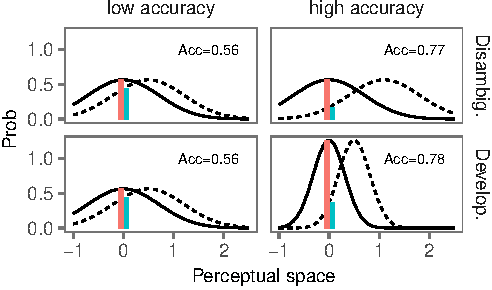
\includegraphics{figs/illus-1} 

}

\caption[An illustration of the probabilistic/continuous account using simulated data]{An illustration of the probabilistic/continuous account using simulated data. A word is represented with a distribution over the perceptual space (indicated in red or blue). When the uncertainty of the representation is large relative to the distance between the stimuli (top panel), an instance of the red category (indicated with a star) could also be a plausible instance of the green category, hence the low recognition accuracy score. The accuracy increases when the stimuli are less similar (left panel), or when the representations are more precise (right panel).}\label{fig:illus}
\end{figure}
\end{CodeChunk}

\section{Model}\label{model}

\subsection{Probabilistic structure}\label{probabilistic-structure}

Our model consists of a set of variables describing the general process
of spoken word recognition in a referential situation. These variables
are related in a way that reflects the simple generative scenario
represented graphically in Figure \ref{fig:model}. When a speaker utters
a sound in the presence of an object, the observer assumes that the
object \(o\) activated the concept \(C\) in the speaker's mind. The
concept prompted the corresponding label \(L\). Finally, the label was
physically instantiated by the sound \(s\).

\begin{SCfigure}
\centering
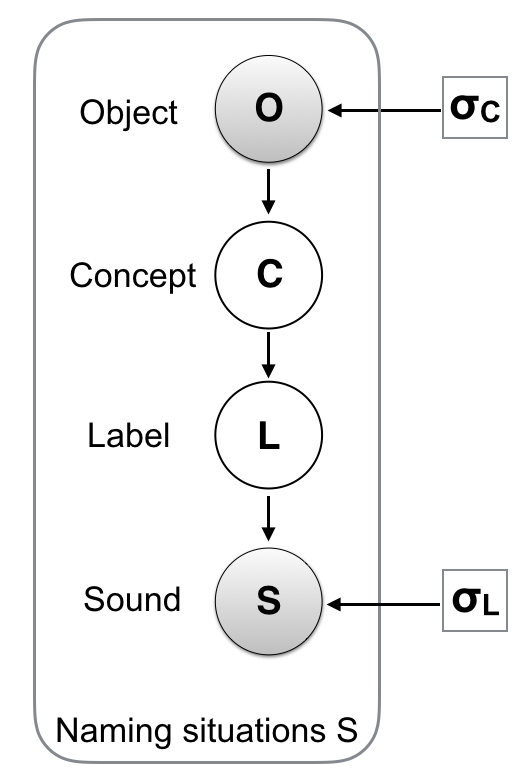
\includegraphics[width=1.5in]{figs/model.png}
\caption{Graphical representation of our model. Circles indicate random variables (shading indicates observed variables). The squares indicate fixed model parameters.}
\label{fig:model}
\end{SCfigure}

A similar probabilistic structure was used by Lewis \& Frank (2013) to
model concept learning, and by Hofer \& Levy (2017) to model spoken word
learning. However, the first study assumed that the sounds are heard
unambiguously, and the second assumed the concepts are observed
unambiguously. In our model, we assume that both labels and concepts are
observed with a certain amount of perceptual noise, which we assume, for
simplicity, is captured by a normal distribution:

\[ p(o | C) \sim  \mathcal{N}(\mu_C, \sigma^2_C) \]
\[ p(s| L) \sim  \mathcal{N}(\mu_L, \sigma^2_L) \] Finally, we assume
there to be one-to-one mappings between concepts and labels and that
observers have successfully learned these mappings during the exposure
phase: \[
P(L_i|C_j) = 
\begin{cases}
  1 & \text{if  }  i=j \\  
  0  & \text{otherwise  }
\end{cases}
\]

\subsection{Inference}\label{inference}

The learner hears a sound \(s\) and has to decide which object \(o\)
provides an optimal match to this sound. To this end, they must compute
the probability \(P(o|s)\) for all possible objects. This probability
can be computed by summing over all possible concepts and labels:
\[P(o|s)=\sum_{C,L} P(o, C, L| s) \propto \sum_{C,L} P(o, C, L, s) \]
The joint probability \(P(o, C, L, s)\) is obtained by factoring the
Bayesian network in Figure \ref{fig:model}:
\[P(o,C,L,s) = P(s|L)P(L|C)P(C|o)P(o) \] which can be transformed using
Bayes rule into:

\[P(o,C,L,s) = P(s|L)P(L|C)P(o|C)P(C) \] Finally, assuming that the
concepts' prior probability is uniformly
distributed\footnote{This is a reasonable assumption in our particular case given the similarity of the concepts used in each naming situation in our experiment.},
we obtain the following expression, where all conditional dependencies
are now well defined:

\begin{equation}
P(o|s) = \frac{\sum_{C,L} P(s|L)P(o|C)P(L|C)}{\sum_{o} \sum_{C,L} P(s|L)P(o|C)P(L|C)}
\end{equation}

\subsection{Task and model
predictions}\label{task-and-model-predictions}

\begin{CodeChunk}
\begin{figure}[t]

{\centering 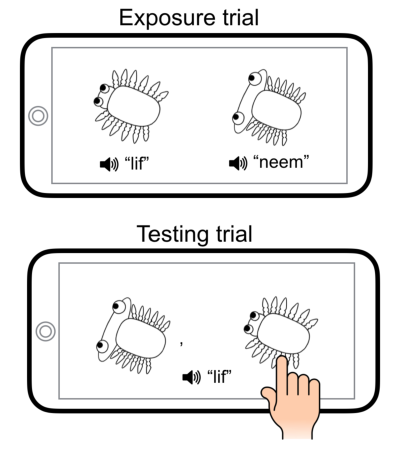
\includegraphics{figs/task-1} 

}

\caption{\label{fig:task}An overview of the task used in this study.}\label{fig:task}
\end{figure}
\end{CodeChunk}

We use the model to predict performance in the word learning task
introduced by Stager \& Werker (1997), with a two-alternative forced
choice as in Yoshida et al. (2009). In this task, participants are first
exposed to the association between pairs of nonsense words (e.g.,
``lif''/``neem'') and pairs of objects. The word-object associations are
introduced sequentially. After this exposure phase, participants perform
a series of test trials. In each of these trials, one of the two sounds
is uttered (e.g., ``lif'') and participants choose the corresponding
object from the two alternatives. An overview of the task is shown in
Figure \ref{fig:task}.

We used Equation 1 and the probability distributions defined above to
obtain the exact analytical expression for the probability of accurate
responses \(p(o_T | s)\) (target object \(o_T\) given a sound \(s\)) in
the simple case of two-alternative forced choice in the testing phase of
our experimental task:

\begin{equation}
P(o_T|s)= \frac{1 + e^{-(\Delta s^2/2\sigma_L^2+ \Delta o^2/2\sigma_C^2)}}{1 + e^{-(\Delta s^2/2\sigma_L^2+ \Delta o^2/2\sigma_C^2)}+ e^{-\Delta s^2 /2\sigma_L^2} + e^{-\Delta o^2 /2\sigma_C^2 }}
\end{equation}

Figure \ref{fig:simulation} show simulations of the predicted accuracy
(Expression 2) as a function of the distinctiveness parameters
(\(\Delta s\) and \(\Delta o\)) and the precision parameters, i.e., the
variances of the distributions \(p(s| L)\) and \(p(o | C)\). To
understand the qualitative behavior of the model, we assumed for
simplicity that the precision parameter has similar values in both
distributions, i.e., \(\sigma =\sigma_C \approx \sigma_L\) (but we will
allow those parameters to vary independently in the rest of the paper).

\begin{CodeChunk}
\begin{figure*}[h]

{\centering 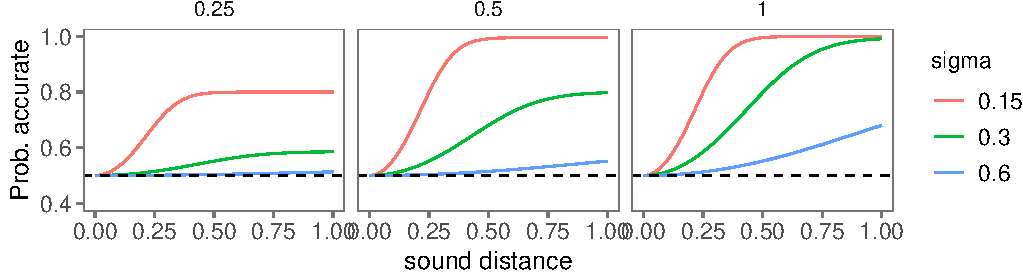
\includegraphics{figs/simulation-1} 

}

\caption{\label{fig:simulation}The predicted probability of accurate responses in the testing phase as a function of stimuli distinctiveness $\Delta s$ and $\Delta o$ and representation precision $\sigma$ (for simplicity, we assume here that $\sigma$=$\sigma_C$=$\sigma_L$). Dashed line represents chance.}\label{fig:simulation}
\end{figure*}
\end{CodeChunk}

The simulations explain some previously documented facts, and make new
predictions:

\begin{enumerate}
\def\labelenumi{\arabic{enumi})}
\item
  For fixed values of \(\Delta o\) and \(\sigma\), the probability of
  accurate responses increases as a function of \(\Delta s\). This
  pattern accounts for the fact that similar sounds are generally more
  challenging to learn than different sounds for both children (Stager
  \& Werker, 1997) and adults (Pajak et al., 2016).
\item
  For fixed values of \(\Delta s\) and \(\Delta o\), accuracy increases
  when the representational uncertainty (characterized with \(\sigma\))
  decreases. This fact may explain development, i.e., younger children
  have noisier representations (see Swingley, 2007; Yoshida et al.,
  2009), which leads to lower word recognition accuracy, especially for
  similar-sounding words.
\item
  For fixed values of \(\Delta s\) and \(\sigma\), accuracy increases
  with the visual distance between the semantic referents \(\Delta o\).
  This is a new prediction that our model makes. Previous work studied
  the effect of several bottom-up and top-down properties in
  disambiguating similar sounding words (e.g., Fennell \& Waxman, 2010;
  Rost \& McMurray, 2009; Thiessen, 2007), but to our knowledge, no
  previous study in the literature tested the effect of the visual
  distance between the semantic referents.
\end{enumerate}

\section{Experiment}\label{experiment}

In this experiment, we tested participants in the word learning task
introduced above (Figure \ref{fig:task}). More precisely, we explored
the predictions related to both distinctiveness and precision. Sound
similarity (\(\Delta s\)) and object similarity (\(\Delta o\)) were
varied simultaneously in a within-subject design. Two age groups
(preschool children and adults) were tested on the same task to explore
whether development can be characterized with the uncertainty
parameters, \(\sigma_C\) and \(\sigma_L\). The experiment, sample size,
exclusion criteria and the model's main predictions were pre-registered.

\subsection{Methods}\label{methods}

\subsubsection{Participants}\label{participants}

We planned to recruit a sample of \(N=60\) children ages 4-5 years from
the Bing Nursery School on Stanford University's campus. Here we report
data from \(N=\) 55 children. An additional \(N=\) 35 children
participated but were removed from analyses because they were not above
chance on the catch trials due to the challenging nature of our
procedure (see below). We also collected a planned sample of \(N=100\)
adult participants through Amazon Mechanical Turk. We planned to exclude
data from participants who did not do well on the catch trials (\(N=\)
26) and from participants who were familiar with the non-English sound
stimuli we used in the adult experiment (\(N=\) 0), yielding a final
sample of \(N=\) 74.

\subsubsection{Stimuli and similarity
rating}\label{stimuli-and-similarity-rating}

The sound stimuli were generated using the MBROLA Speech Synthesizer
(Dutoit, Pagel, Pierret, Bataille, \& Van der Vrecken, 1996). We
generated three kinds of nonsense word pairs which varied in their
degree of similarity to English speakers: 1) ``different'':
``lif''/``neem'' and ``zem''/``doof'', 2) ``intermediate'':
``aka''/``ama'' and ``ada''/``aba'', and 3) ``similar'' non-English
minimal pairs: ``ada''/``a\textipa{d\super h}a'' (in hindi) and
``a\textipa{Q}a''/``a\textipa{\textcrh}a'' (in arabic).

As for the objects, we used the Dynamic Stimuli javascript
library\footnote{https://github.com/erindb/stimuli} which allowed us to
generate objects in four different categories: ``tree'', ``bird'',
``bug'', and ``fish''. These categories are supposed to be naturally
occurring kinds that might be seen on an alien planet. In each category,
we generated ``different'', ``intermediate'' and ``similar'' pairs by
manipulating a continuous property controlling features of the
category's shape (e.g, body stretch or head fatness).

In a separate survey, \(N=20\) participants recruited on Amazon
Mechanical Turk evaluated the similarity of each sound and object pair
on a 7-point scale. We scaled responses within the range {[}0,1{]}. Data
are shown in Figure \ref{fig:stim}, for each stimulus group. These data
will be used in the models as the perceptual distance of sound pairs
(\(\Delta s\)) and object pairs (\(\Delta o\)).

\subsubsection{Design}\label{design}

Each age group saw only two of the three levels of similarity described
in the previous sub-section: ``different'' vs. ``intermediate'' for
preschoolers and ``intermediate'' vs. ``similar'' for adults. We made
this choice in light of pilot studies showing that adults were at
ceiling with ``different'' sounds/objects, and children were at chance
with the ``similar'' sounds/objects. That said, this difference in the
level of similarity is accounted for in the model by using the
appropriate perceptual distance used in each age group (Figure
\ref{fig:stim}).

\begin{CodeChunk}
\begin{figure}[h]

{\centering 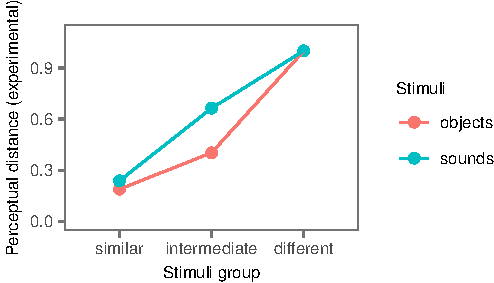
\includegraphics{figs/stim-1} 

}

\caption{\label{fig:stim}Distances for both sound and object pairs from an adult norming study. Data represent Likert values normalized to [0,1] interval. Error bars represent 95\% confidence intervals.}\label{fig:stim}
\end{figure}
\end{CodeChunk}

To maximize our ability to measure subtle stimulus effects, the
experiment was a 2x2 within-subjects factorial design with four
conditions: high/low sound similarity crossed with high/low visual
object similarity. Besides the 4 conditions, we also tested participants
on a fifth catch condition which was similar in its structure to the
other ones but was used only to select participants who were able to
follow the instructions and show minimal learning.

\subsubsection{Procedure}\label{procedure}

Preschoolers were tested at the nursery school using a tablet, whereas
adults used their own computers to complete the same experiment online.
Participants were tested in a sequence of five conditions: the four
experimental conditions plus the catch condition. In each condition,
participants saw a first block of four exposure trials followed by four
testing trials, and a second block of two exposure trials (for memory
refreshment) followed by an additional four testing trials. The length
of this procedure was demanding, especially for children, but we adopted
a fully within-subjects design based on pilot testing that indicated
that precision of measurement was critical for testing our experimental
predictions.

\begin{CodeChunk}
\begin{figure*}[h]

{\centering 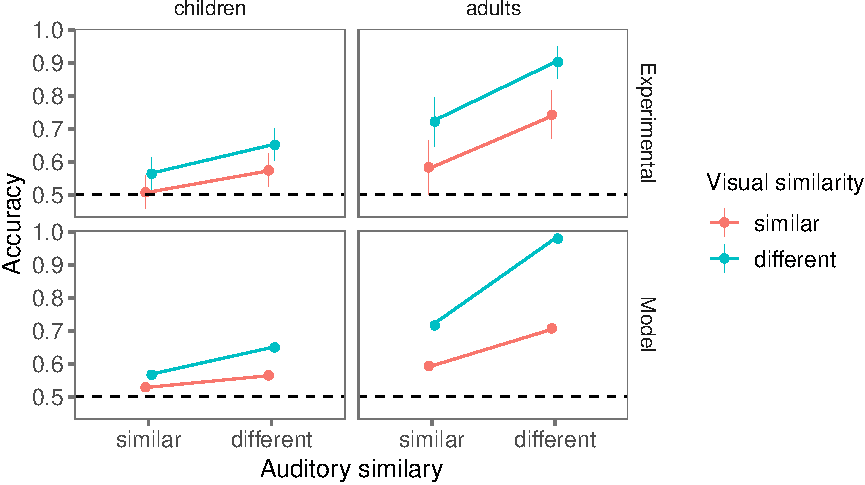
\includegraphics{figs/all_data-1} 

}

\caption{\label{fig:data_all}Accuracy of novel word recognition as a function of the sound distance, the object distance, and the age group (preschool children vs. adults). We show both the models' predictions (dashed lines) and the experimental results (solid lines). The single-variance model uses one joint fitting parameter for both sound and meaning variances. The double-variance model uses two separate fittings parameters for the sound and the meaning variances. Error bars represent 95\% confidence intervals.}\label{fig:all_data}
\end{figure*}
\end{CodeChunk}

In the exposure trials, participants saw two objects associated with
their corresponding sounds. We presented the first object on the left
side of the tablet's screen simultaneously with the corresponding sound.
The second sound-object association followed on the other side of the
screen after 500ms. For both objects, visual stimuli were present for
the duration of the sound clip (∼800ms). In the testing trials,
participants saw both objects simultaneously and heard only one sound.
They completed the trial by selecting which of the two objects
corresponded to the sound. The object-sound pairings were randomized
across participants, as was the order of the conditions (except for the
catch condition which was always placed in the middle of the testing
sequence). We also randomized the on-screen position (left vs.~right) of
the two pictures on each testing trial.

\subsection{Results}\label{results}

We first analyzed the results using a mixed-effects logistic regression
with sound distance, object distance and age group as fixed effects, and
with a maximal random effects structure (allowing us to take into
account the full nested structure of our data) (Barr, Levy, Scheepers,
\& Tily, 2013). We found main effects for all the fixed effects in the
regression. For the sound distance, we obtained \(\beta =\) 0.52 (\(p\)
\textless{} 0.001), replicating previous findings. For object distance,
we found \(\beta =\) 0.83 (\(p\) \textless{} 0.001), and this finding
confirms the new prediction of our model. Finally, for the age group, we
obtained \(\beta =\) 0.76 (\(p\) \textless{} 0.001), showing that
performance improves with age.

We next fit our model (using Equation 2) to the participants' responses
in each age group using non-linear least-squares. The values of
\(\Delta s\) and \(\Delta o\) were set based on data from the similarity
judgment task (Figure \ref{fig:stim}). The model has two degrees of
freedom for each group, i.e., \(\sigma_C\) and \(\sigma_L\). We call it
the double-variance model. Figure \ref{fig:data_all} (dashed lines)
shows the predictions. The double-variance model captures the behavioral
patterns in both age groups: starting from a low accuracy recognition
when both the sound and object distances are small, the model correctly
predicts an increase in accuracy when either the sound distance or the
object distance increases. Further, accuracy is correctly predicted to
be maximal when both the sound and object distances are high.

The values of the parameters were as follows. Children had a
label-specific uncertainty of \(\sigma_S =\) 0.83 {[}0.64,
1.02{]}\footnote{All uncertainty intervals in this paper represent 95\% Confidence Intervals.},
and a concept-specific uncertainty of \(\sigma_C =\) 0.31 {[}0.11,
0.51{]}. Adults had a label-specific uncertainty of \(\sigma_S =\) 0.12
{[}0.12, 0.13{]}, and a concept-specific uncertainty of \(\sigma_C =\)
0.17 {[}0.16, 0.18{]}. As predicted, the uncertainty parameters were
larger for children than they were for adults, showing that the
probabilistic representations becomes more refined (that is, \(\sigma\)
becomes smaller) across development. The developmental effect was more
important for the label-specific uncertainty.

The double-variance model explained almost all the variance in the
participants' mean responses. To investigate whether the model's strong
predictive power was due to overfitting, we fit a simplified version
with only one degree of freedom (i.e., a single variance common to both
sounds and objects). This single-variance model also captured the main
qualitative patterns and remained highly predictive (\(R^2=\) 0.95).
This result suggests that the explanatory power of the model is largely
due to its structure, rather than its degrees of freedom.

\section{General Discussion}\label{general-discussion}

This paper explored the idea that some seemingly stage-like patterns in
cognitive development can be characterized in a continuous fashion. We
used as a case study the seminal work of Stager \& Werker (1997) showing
a discrepancy between children's speech perception abilities and their
word learning skills. While much of the previous investigation of this
finding has been interested in the source of this discrepancy, here we
have explored how it could arise from continuous developmental change in
perceptual uncertainty.

Building on some previous discussions (e.g., Swingley, 2007; Yoshida et
al., 2009), we proposed a model where perceptual stimuli are encoded
probabilistically. We tested the model's predictions against data
collected from preschool children and adults and we showed that
developmental changes in word-object mappings can indeed be
characterized as a continuous refinement (i.e., uncertainty reduction)
in qualitatively similar representations across the life span.

The model made a new prediction which we tested experimentally: Learning
similar words is not only modulated by the similarity of their
phonological forms, but also by the visual similarity of their semantic
referents. More generally, since visual similarity is an early
organizing feature in the semantic domain (e.g., Wojcik \& Saffran,
2013), our finding suggests that children may prioritize the acquisition
of words that are quite distant in the semantic space. This suggestion
is supported by recent findings based on the investigation of early
vocabulary growth (Engelthaler \& Hills, 2017; Sizemore, Karuza, Giusti,
\& Bassett, 2018).

One limitation of this work is that the model was fit to data from
children at a relatively older age (4-5 years old) than what is
typically studied in the literature (14-18 month-old). We selected this
older age group to optimize the number and precision of the experimental
measures (both are crucial to model fitting). Data collection involved
presenting participants with several trials across four conditions in a
between-subject design. It would have been challenging to obtain such
measures with infants.

In sum, this paper proposes a model that accounts for the development of
an important aspect of word learning. Our account suggests that the
developmental data can be explained based on a continuous process
operating over similar representations across development, suggesting
developmental continuity. We used a case from word learning as an
example, but the same idea might apply to other aspects of cognitive
development that are typically thought of as stage-like (e.g.,
acquisition of a theory of mind). Computational models, such as the one
proposed here, can help us investigate the extent to which such
discontinuities emerge due to genuine qualitative changes and the extent
to which they reflect the granularity of the researchers' own
measurement tools.

\vspace{1em}

\fbox{\parbox[b][][c]{7.3cm}{\centering All data and code are available online at\ \url{https://github.com/afourtassi/kidswitch} }}
\vspace{1em}

\section{References}\label{references}

\setlength{\parindent}{-0.1in} \setlength{\leftskip}{0.125in} \noindent

\hypertarget{refs}{}
\hypertarget{ref-barr2013}{}
Barr, D., Levy, R., Scheepers, C., \& Tily, H. (2013). Random effects
structure for confirmatory hypothesis testing: Keep it maximal.
\emph{Journal of Memory and Language}, \emph{68}(3).

\hypertarget{ref-carey2009}{}
Carey, S. (2009). \emph{The origin of concepts}. Oxford University
Press.

\hypertarget{ref-dutoit1996}{}
Dutoit, T., Pagel, V., Pierret, N., Bataille, F., \& Van der Vrecken, O.
(1996). The mbrola project: Towards a set of high quality speech
synthesizers free of use for non commercial purposes. In
\emph{Proceedings of ICSLP} (Vol. 3). IEEE.

\hypertarget{ref-engelthaler2017}{}
Engelthaler, T., \& Hills, T. T. (2017). Feature biases in early word
learning: Network distinctiveness predicts age of acquisition.
\emph{Cognitive Science}, \emph{41}.

\hypertarget{ref-fennell2010}{}
Fennell, C., \& Waxman, S. (2010). What paradox? Referential cues allow
for infant use of phonetic detail in word learning. \emph{Child
Development}, \emph{81}.

\hypertarget{ref-hofer2017}{}
Hofer, M., \& Levy, R. (2017). Modeling Sources of Uncertainty in Spoken
Word Learning. In \emph{Proceedings of the 39th Annual Meeting of the
Cognitive Science Society}.

\hypertarget{ref-lewis2013}{}
Lewis, M., \& Frank, M. (2013). An integrated model of concept learning
and word-concept mapping. In \emph{Proceedings of the annual meeting of
the cognitive science society} (Vol. 35).

\hypertarget{ref-pajak2016}{}
Pajak, B., Creel, S., \& Levy, R. (2016). Difficulty in learning
similar-sounding words: A developmental stage or a general property of
learning? \emph{Journal of Experimental Psychology: Learning, Memory,
and Cognition}, \emph{42}(9).

\hypertarget{ref-piaget1954}{}
Piaget, J. (1954). \emph{The construction of reality in the child}. New
York, NY, US: Basic Books.

\hypertarget{ref-rost2009}{}
Rost, G., \& McMurray, B. (2009). Speaker variability augments
phonological processing in early word learning. \emph{Developmental
Science}, \emph{12}.

\hypertarget{ref-sizemore2018}{}
Sizemore, A. E., Karuza, E. A., Giusti, C., \& Bassett, D. S. (2018).
Knowledge gaps in the early growth of semantic feature networks.
\emph{Nature Human Behaviour}, \emph{2}(9).

\hypertarget{ref-stager1997}{}
Stager, C., \& Werker, J. (1997). Infants listen for more phonetic
detail in speech perception than in word-learning tasks. \emph{Nature},
\emph{388}(6640).

\hypertarget{ref-swingley2007}{}
Swingley, D. (2007). Lexical exposure and word-form encoding in
1.5-year-olds. \emph{Developmental Psychology}, \emph{43}(2).

\hypertarget{ref-thiessen2007}{}
Thiessen, E. (2007). The effect of distributional information on
children's use of phonemic contrasts. \emph{Journal of Memory and
Language}, \emph{56}.

\hypertarget{ref-werker2002}{}
Werker, J., Fennell, C., Corcoran, K., \& Stager, C. (2002). Infants'
ability to learn phonetically similar words: Effects of age and
vocabulary size. \emph{Infancy}, \emph{3}.

\hypertarget{ref-white2013}{}
White, K., Yee, E., Blumstein, S., \& Morgan, J. (2013). Adults show
less sensitivity to phonetic detail in unfamiliar words, too.
\emph{Journal of Memory and Language}, \emph{68}(4).

\hypertarget{ref-wojcik2013}{}
Wojcik, E., \& Saffran, J. (2013). The ontogeny of lexical networks:
Toddlers encode the relationships among referents when learning novel
words. \emph{Psychological Science}, \emph{24}(10).

\hypertarget{ref-yoshida2009}{}
Yoshida, K., Fennell, C., Swingley, D., \& Werker, J. (2009).
14-month-olds learn similar-sounding words. \emph{Developmental
Science}, \emph{12}.

\end{document}
